% -*- latex -*-
%%%%%%%%%%%%%%%%%%%%%%%%%%%%%%%%%%%%%%%%%%%%%%%%%%%%%%%%%%%%%%%%
%%%%%%%%%%%%%%%%%%%%%%%%%%%%%%%%%%%%%%%%%%%%%%%%%%%%%%%%%%%%%%%%
%%%%
%%%% This text file is part of the lecture slides for
%%%% `Parallel Computing'
%%%% by Victor Eijkhout, copyright 2012-2020
%%%%
%%%% SPMD-slides.tex : slides about MPI's SPMD mode
%%%%
%%%%%%%%%%%%%%%%%%%%%%%%%%%%%%%%%%%%%%%%%%%%%%%%%%%%%%%%%%%%%%%%
%%%%%%%%%%%%%%%%%%%%%%%%%%%%%%%%%%%%%%%%%%%%%%%%%%%%%%%%%%%%%%%%

\begin{frame}[containsverbatim]{Overview}
  In this section you will learn how to think about parallelism in
  MPI.

  Commands learned:
  \begin{itemize}
  \item
    \indexmpishow{MPI_Init}, \indexmpishow{MPI_Finalize},
  \item 
    \indexmpishow{MPI_Get_processor_name}, \indexmpishow{MPI_Comm_size}, \indexmpishow{MPI_Comm_rank}
  \end{itemize}
\end{frame}

\sectionframe{The MPI worldview: SPMD}

\frame{\frametitle{Computers when MPI was designed}
  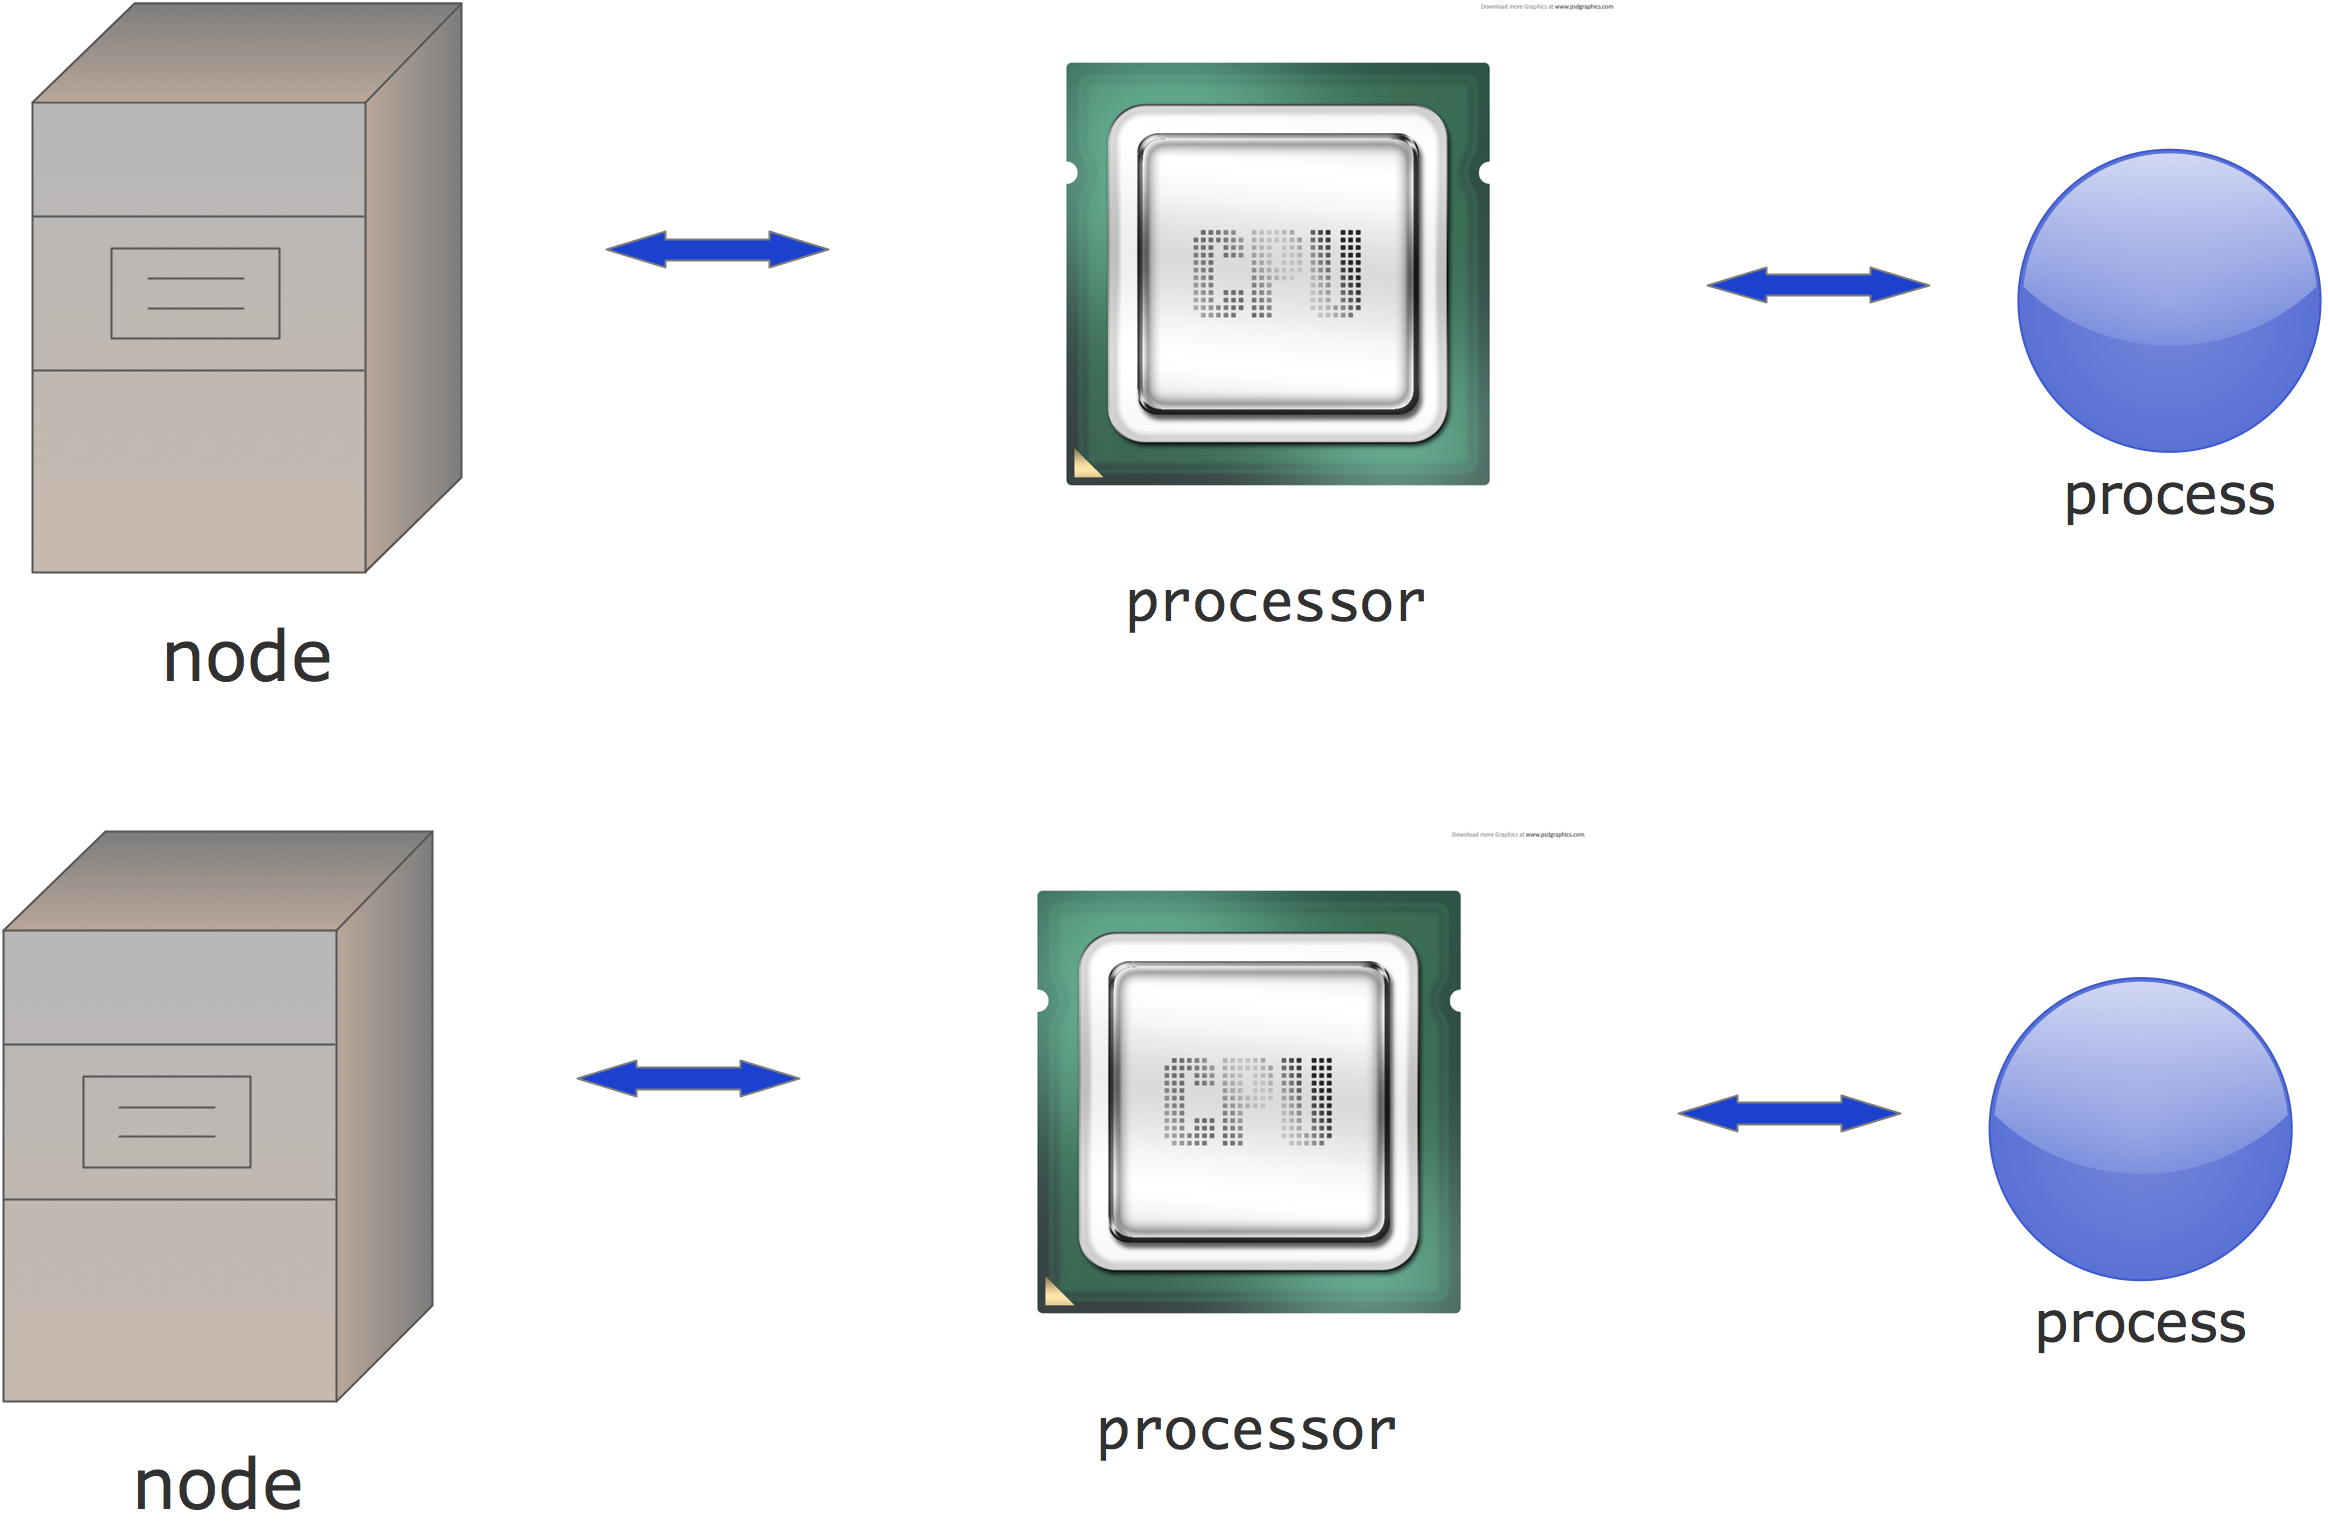
\includegraphics[scale=.1]{mpi-node1}

  One processor and one  process per node;\\
  all communication goes through the network.
}

\frame{\frametitle{Pure MPI}
  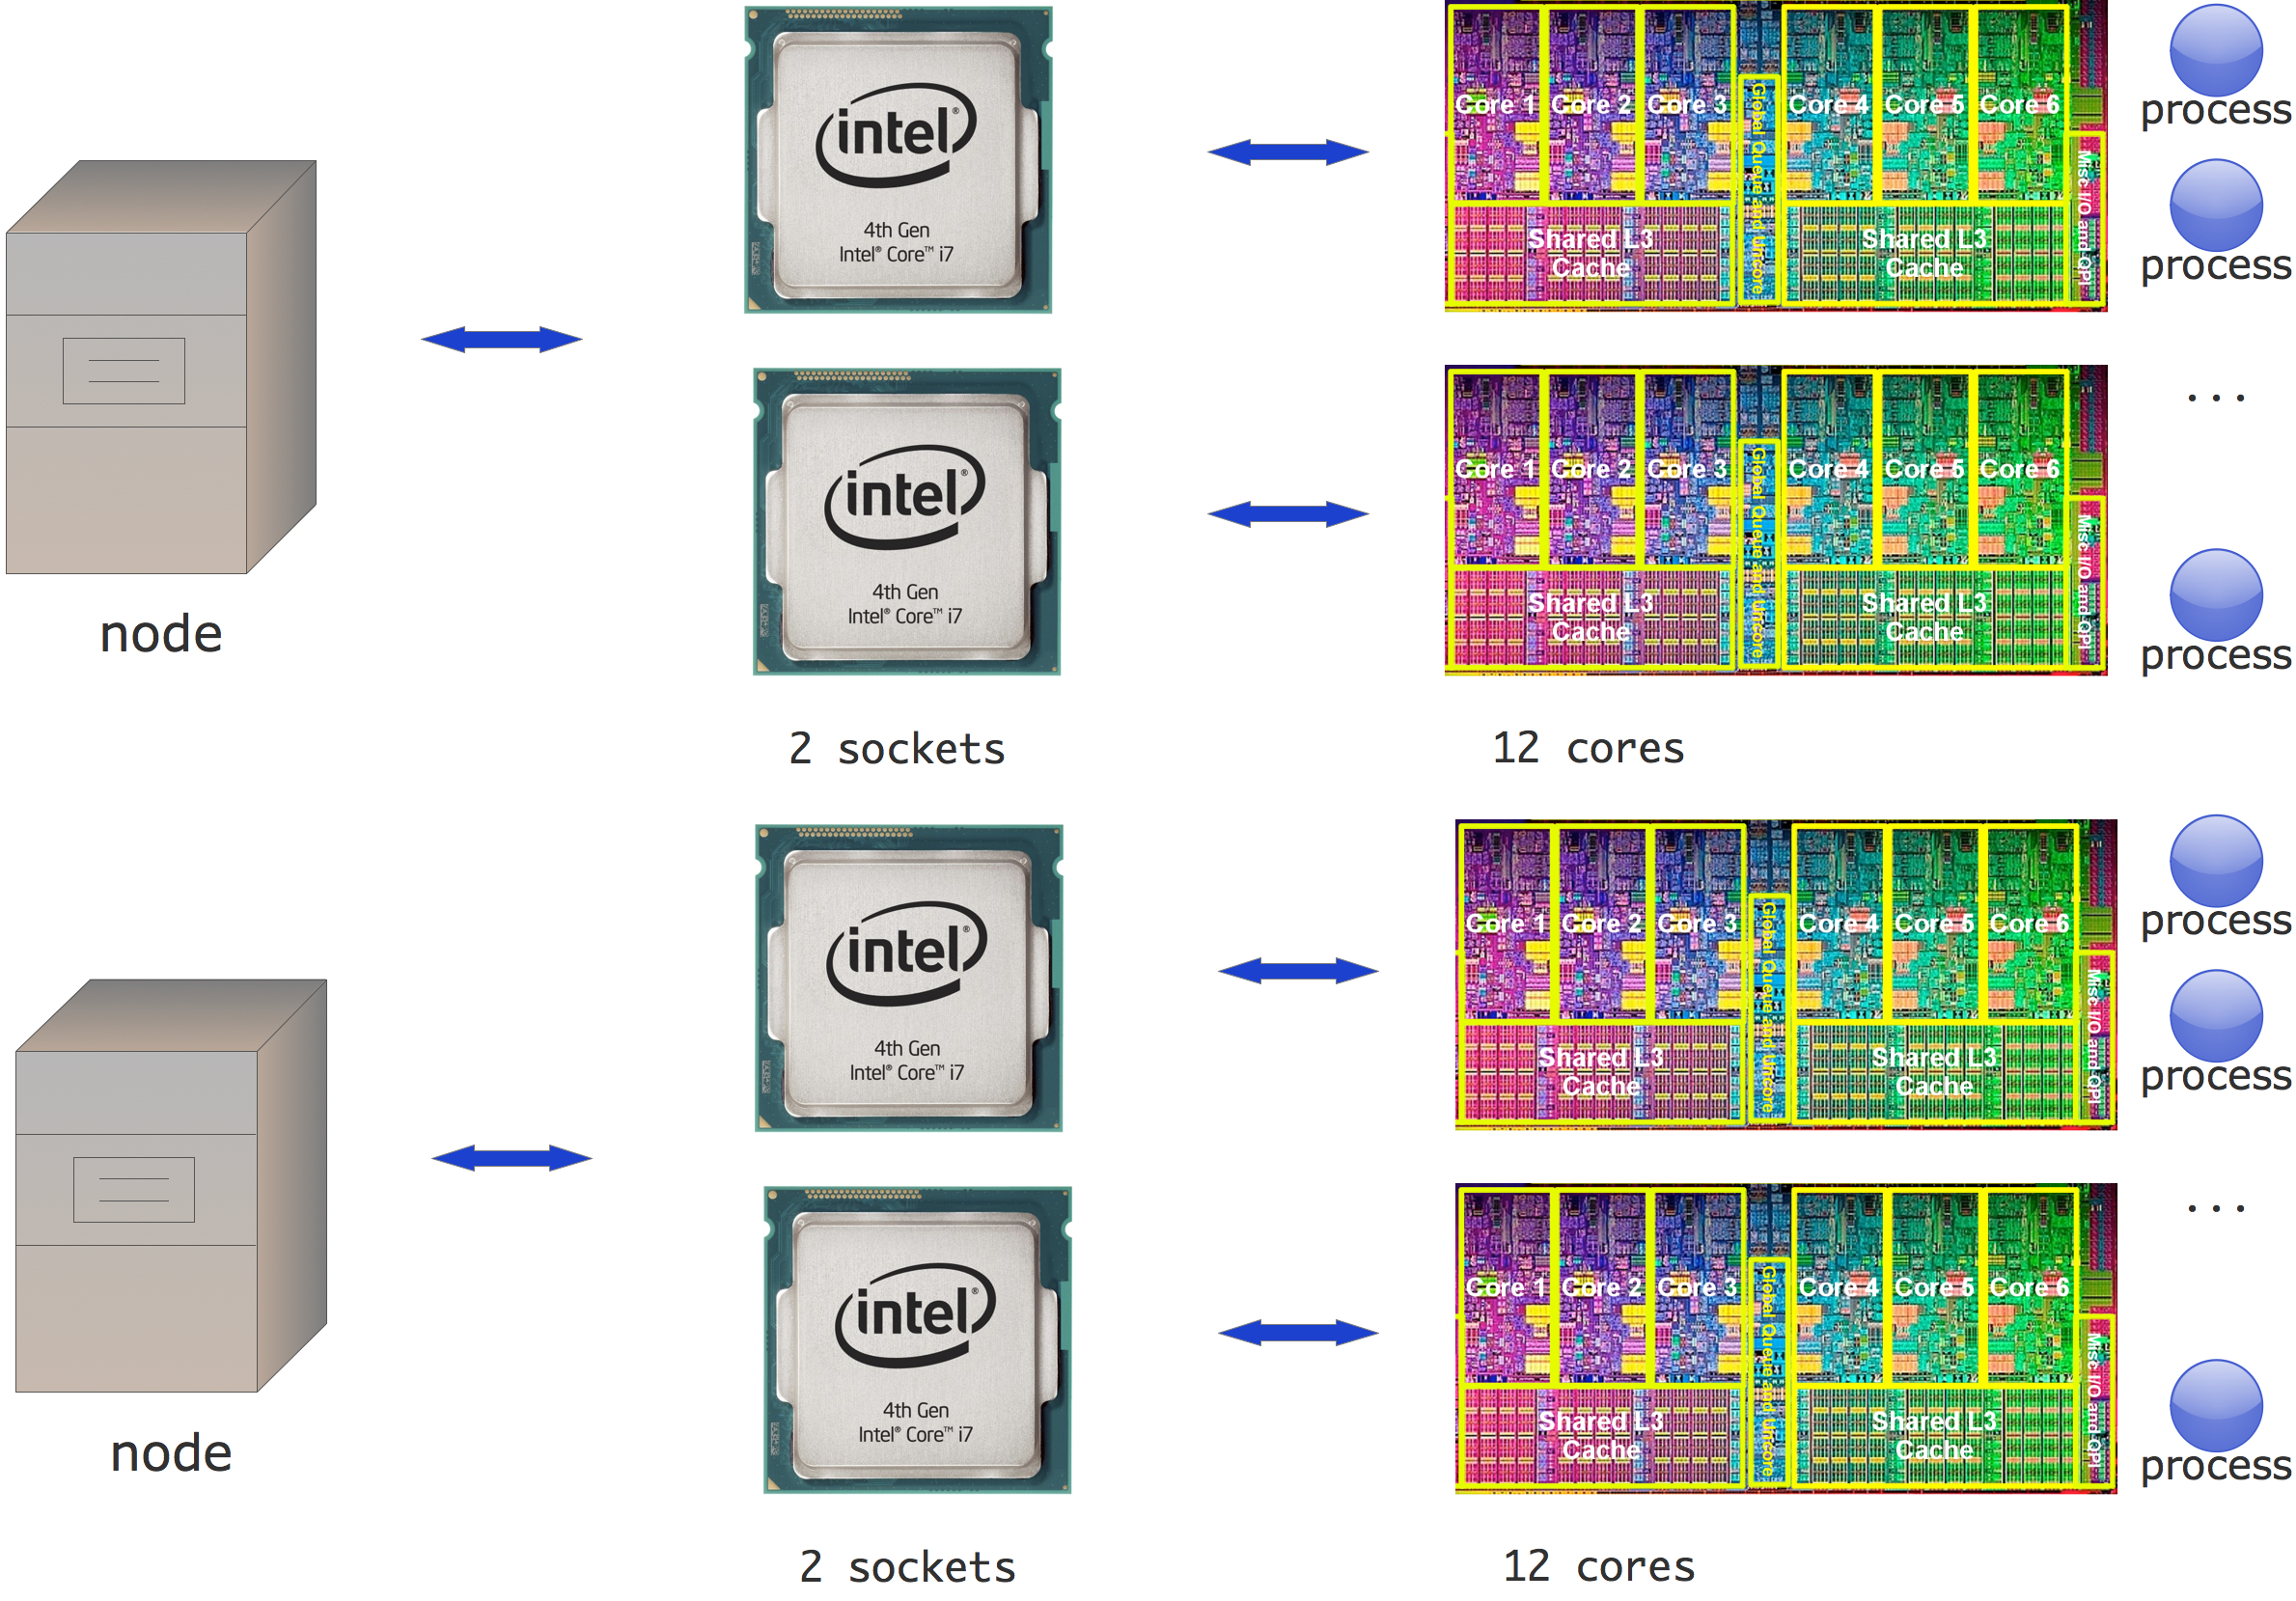
\includegraphics[scale=.1]{mpi-node2}

  A node has multiple sockets, each with multiple cores.\\
  Pure MPI puts a process on each core: pretend shared memory doesn't exist.
}

\frame{\frametitle{Hybrid programming}
  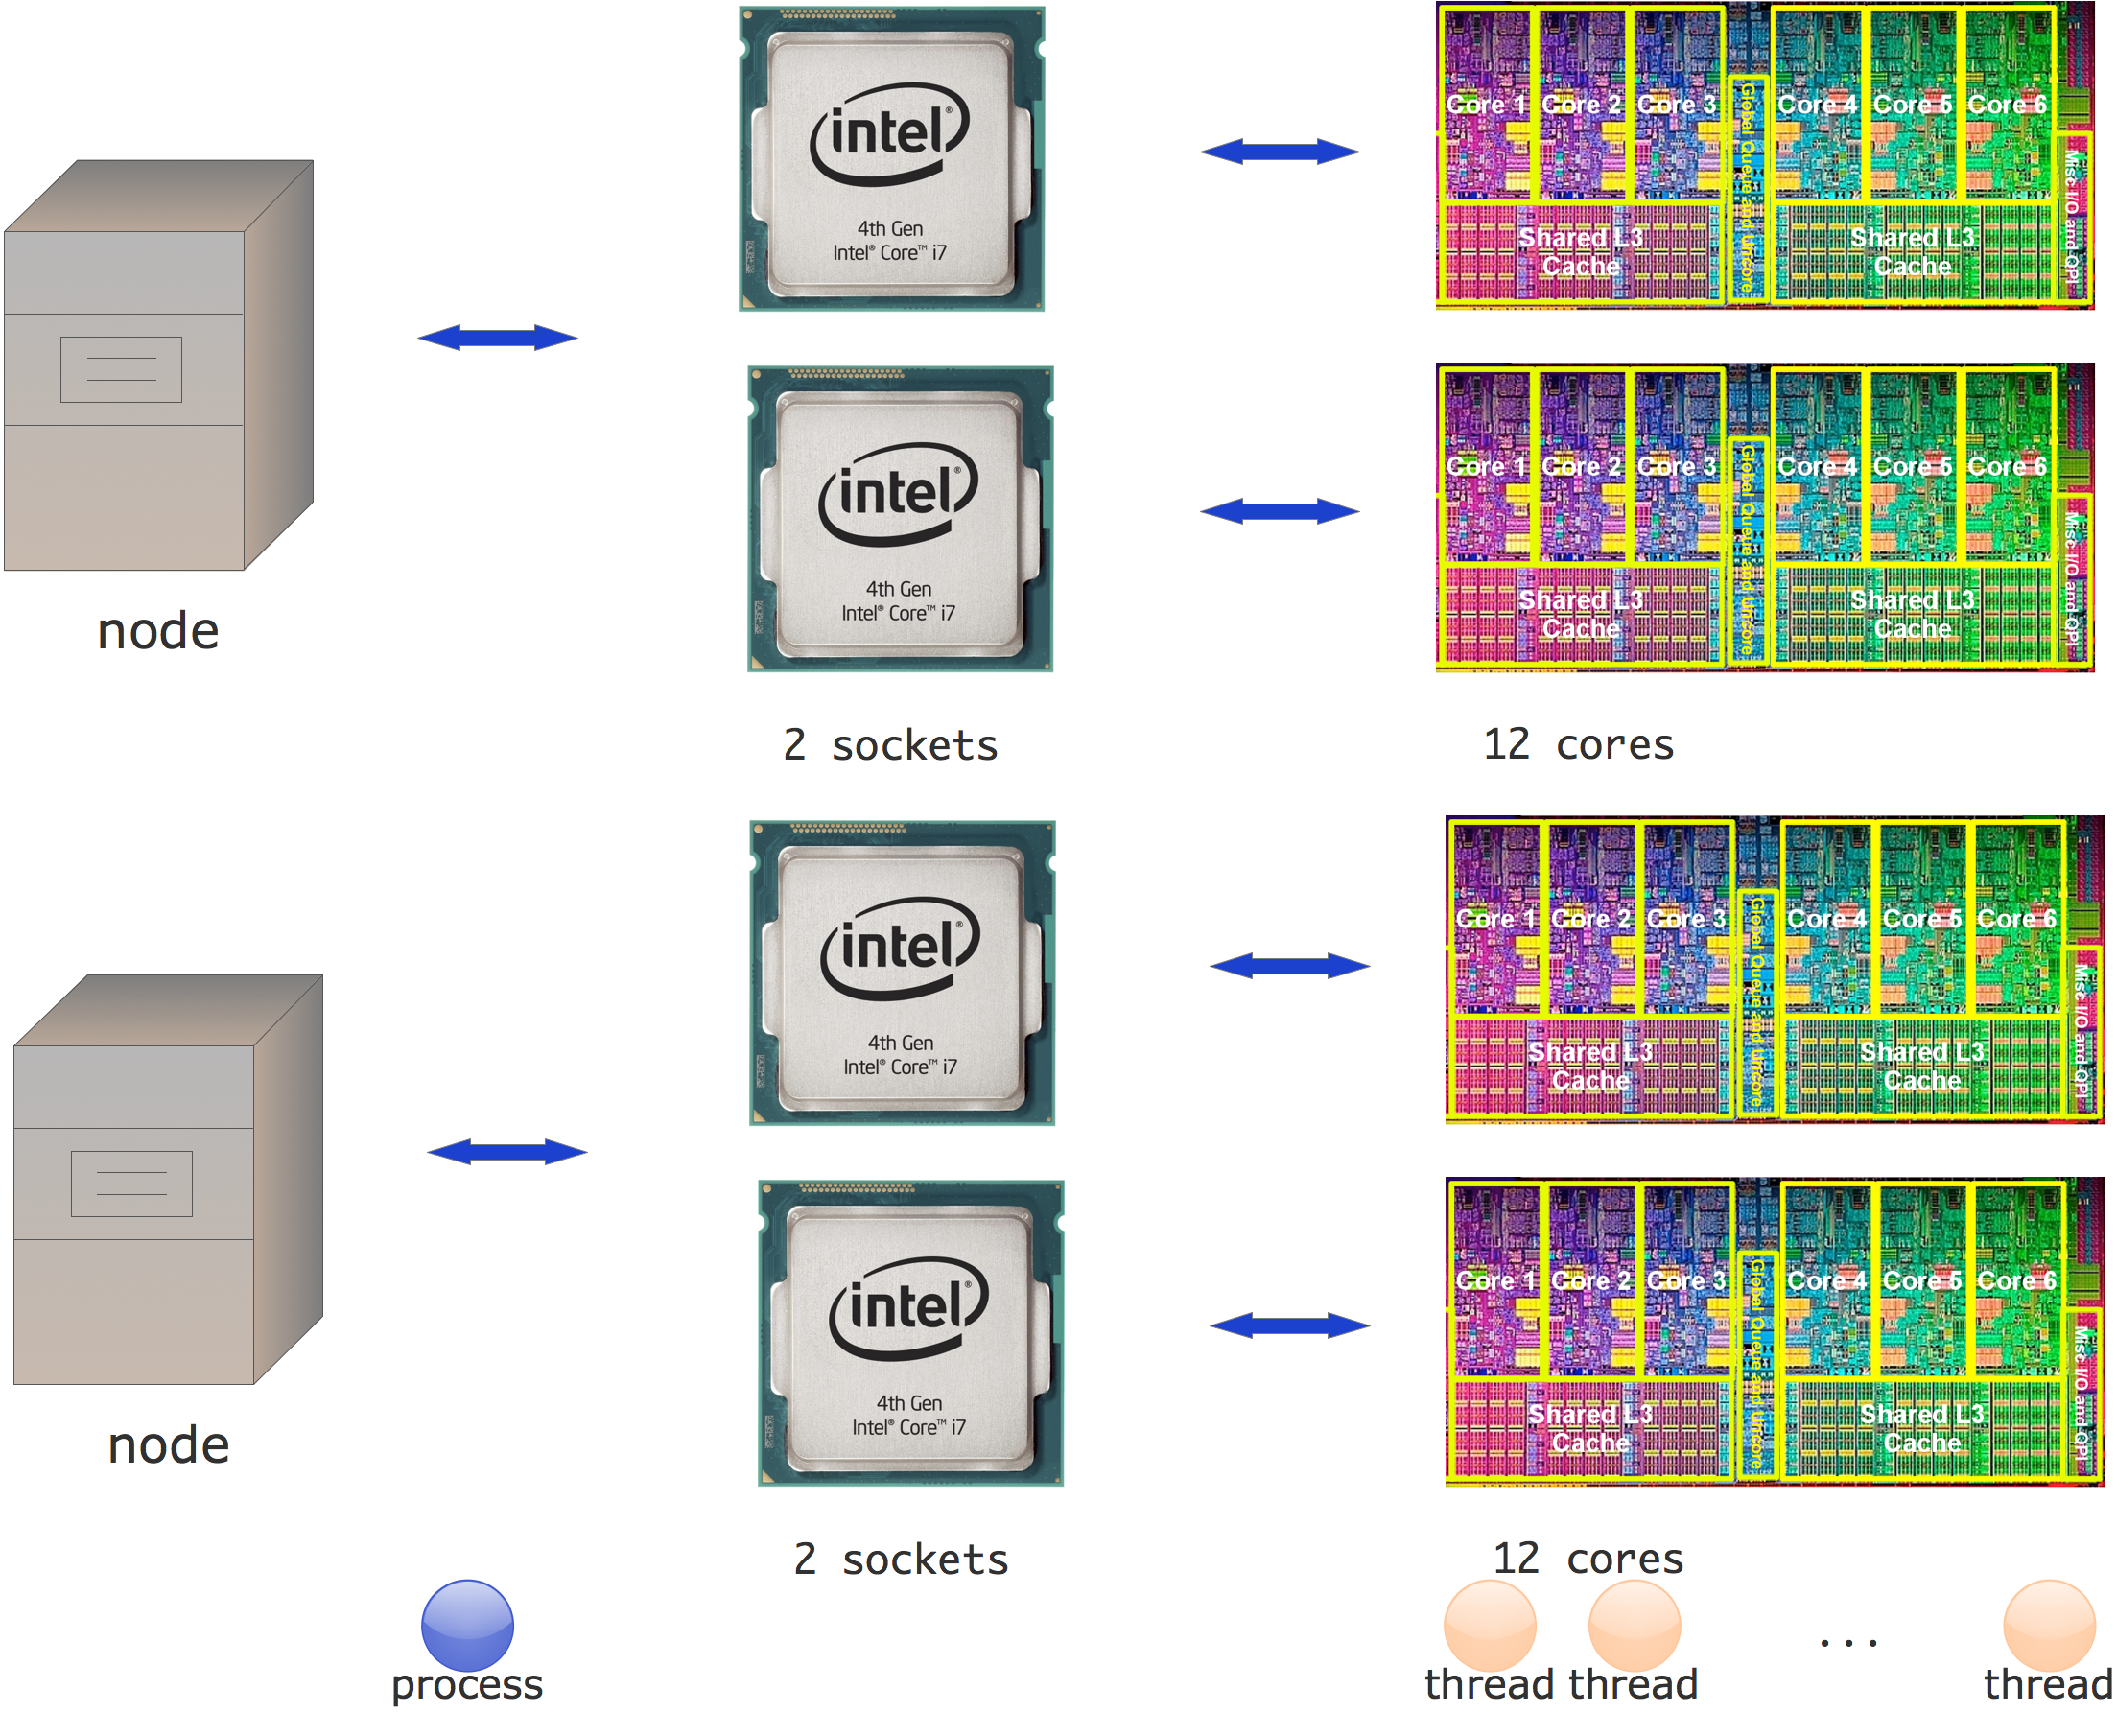
\includegraphics[scale=.1]{mpi-node3}

  Hybrid programming puts a process per node or per socket;\\
  further parallelism comes from threading.\\
  Not in this course\ldots
}

\begin{frame}{Terminology}
  `Processor' is ambiguous: is that a chip or one independent
  instruction processing unit?
  \begin{itemize}
  \item Socket: the processor chip
  \item Processor: we don't use that word
  \item Core: one instruction-stream processing unit
  \item Process: preferred terminology in talking about MPI.
  \end{itemize}  
\end{frame}

\frame{\frametitle{SPMD}
  The basic model of MPI is\\
  `Single Program Multiple Data':\\
  each process is an instance of the same program.

  Symmetry: There is no `master process', all processes are equal,
  start and end
  at the same time.

  Communication calls do not see the cluster structure:\\
  data sending/receiving is the same for all neighbours.
}

\sectionframe{Practicalities}

\begin{frame}[containsverbatim]{Compiling and running}
  MPI compilers are usually called \indextermtt{mpicc},
  \indextermtt{mpif90}, \indextermtt{mpicxx}.

  These are not separate compilers,
  but scripts around the regular C/Fortran compiler. You can use all
  the usual flags.

  Run your program with something like
\begin{verbatim}
mpiexec -n 4 hostfile ... yourprogram arguments
mpirun -np 4 hostfile ... yourprogram arguments
\end{verbatim}
\begin{online}
  Check your local installation!
\end{online}
\begin{tacc}
  At TACC:\\
  \verb+ibrun yourprog+\\
  the number of processes is determined by SLURM.
\end{tacc}
\end{frame}

\begin{frame}[containsverbatim]{Do I need a supercomputer?}
  \begin{itemize}
  \item With \n{mpiexec} and such, you start a bunch of processes that
    execute your MPI program.
  \item Does that mean that you need a cluster or a big multicore?
  \item No! You can start a large number of MPI processes, even on
    your laptop. The OS will use `time slicing'.
  \item Of course it will not be very efficient\ldots
  \end{itemize}
\end{frame}

\begin{frame}{Cluster setup}
  \small
  Typical cluster:
  \begin{itemize}
  \item Login nodes, where you ssh into; usually shared with 100 (or
    so) other people. You don't run your parallel program there!
  \item Compute nodes: where your job is run. They are often exclusive
    to you: no other users getting in the way of your program.
  \end{itemize}
  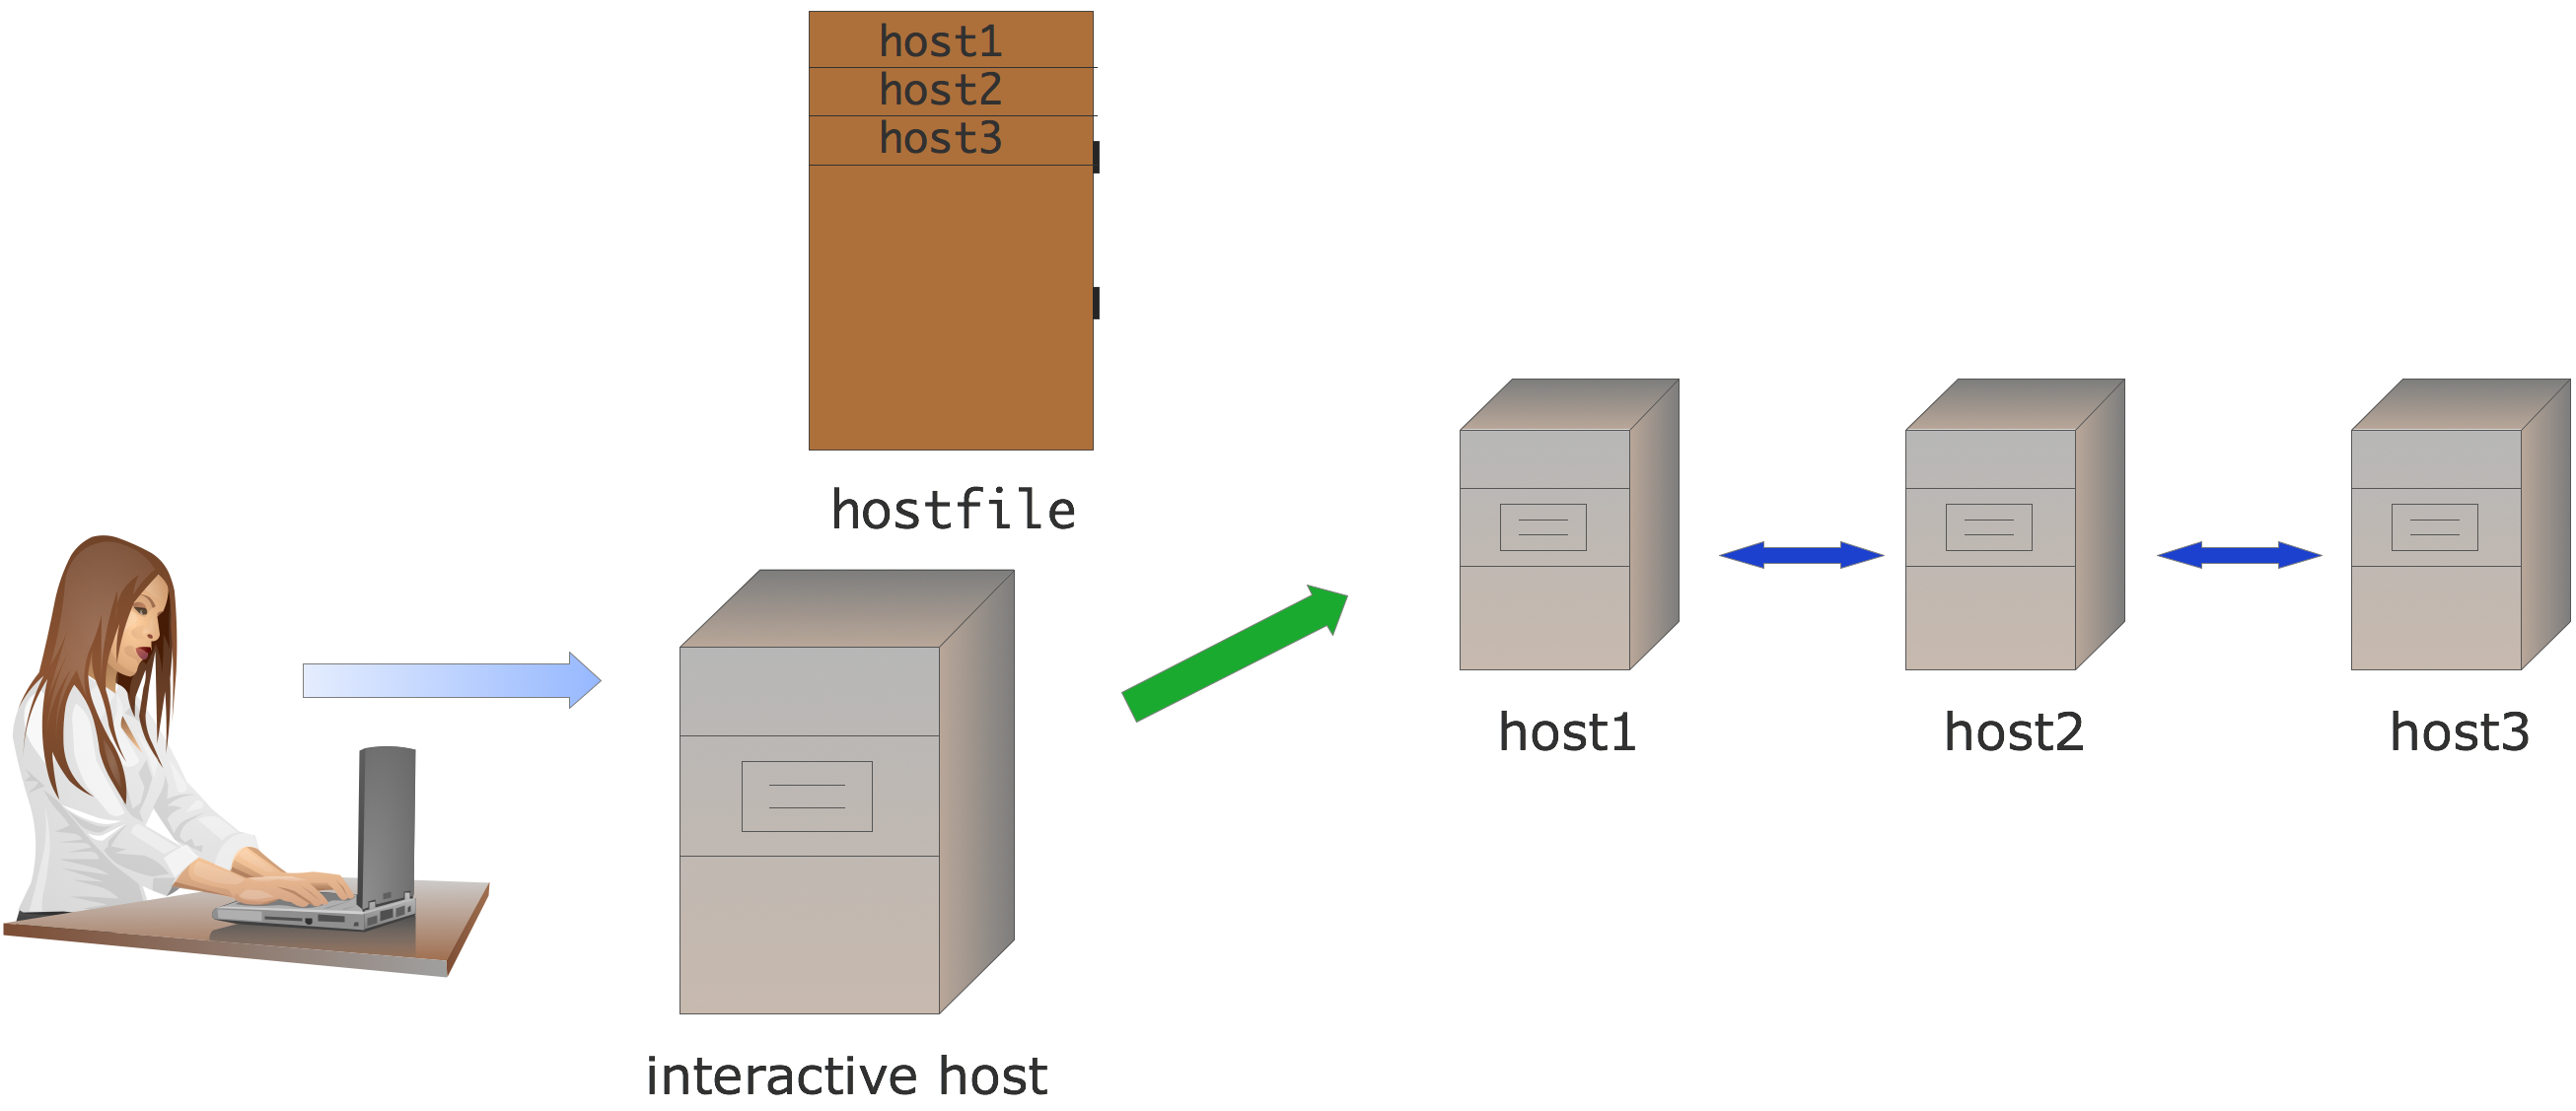
\includegraphics[scale=.08]{graphics/mpi-interactive}

  Hostfile: the description of where your job runs. Usually generated
  by a \indexterm{job scheduler}.
\end{frame}

\begin{comment}
  \begin{tacc}
    \begin{frame}[containsverbatim]{Lab setup}
      \textbf{Official version}:\\
      Open two windows on stampede.
      \begin{itemize}
      \item In one window you will be editing and compiling;
      \item in the other, type \n{idev -N 2 -n 32 -t 4:0:0 } which gives
        you an interactive session of 2~nodes, 32~cores, for the next
        4~hours.
      \end{itemize}
      The C compiler is \texttt{mpicc}, C++ is \texttt{mpicxx}, Fortran is
      \texttt{mpif90}. To run (on a compute node!) type \texttt{ibrun
        yourprog}.

      No hostfiles or process count needed!

      \textbf{Shortcut for training}:\\ issue \n{idev} command, then \n{source
        ~train00/tacc_hpc_sourceme} in idev session.
    \end{frame}
  \end{tacc}
\end{comment}

\begin{frame}[containsverbatim]{How to make exercises}
  \begin{itemize}
  \item Directory: \n{exercises-mpi-c} or \n{cxx} or \n{f} or \n{f08}
    or \n{p}
  \item If a slide has a \n{(exercisename)} over it, there will be a
    template program \n{exercisename.c} (or \n{F90} or \n{py}).
  \item Type \n{make exercisename} to compile it
  \item Python: setup once per session
\begin{verbatim}
module load python2 # or python3
\end{verbatim}
No compilation needed. Run:
\begin{verbatim}
  ibrun python2 yourprogram # or python3
\end{verbatim}
\item Add an exercise of your own to the makefile: add the name to
    the \n{EXERCISES}
  \end{itemize}
\end{frame}

\begin{exerciseframe}[hello]
  \input ex:hello1
\end{exerciseframe}

\begin{frame}{In a picture}
  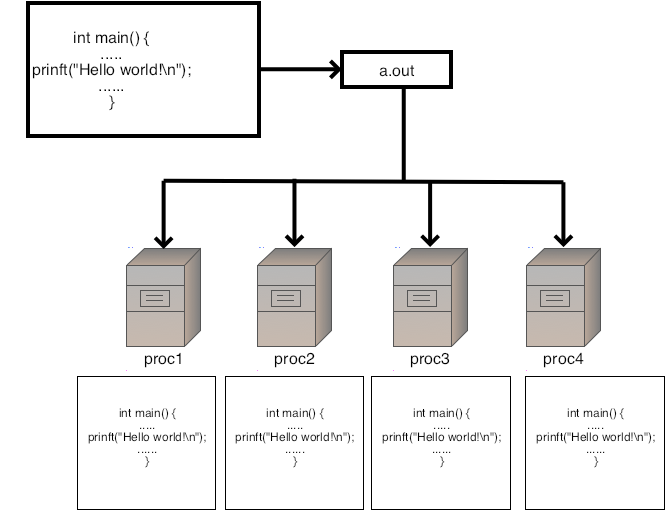
\includegraphics[scale=.45]{hello-parallel}
\end{frame}

\sectionframe{We start learning MPI!}

\begin{mpithree}
\begin{frame}[containsverbatim]{MPI definitions}
You need an include file:
\begin{verbatim}
#include "mpi.h" // for C
use mpi       ! for Fortran90
use mpi_f08   ! for Fortran2008
\end{verbatim}
\begin{itemize}
\item There are no real C++ bindings.
\item True Fortran bindings as of the 2008 standard.
\begin{tacc}
Provided in Intel compiler:
\begin{verbatim}
module load intel/18.0.2
\end{verbatim}
or newer. Not in gcc7.
\end{tacc}
\end{itemize}
\end{frame}

\begin{frame}[containsverbatim]{MPI Init / Finalize}
Then put these calls around your code:
\lstset{language=C}
\begin{lstlisting}
ierr = MPI_Init(&argc,&argv); // zeros allowed
// your code
ierr = MPI_Finalize();  
\end{lstlisting}
and for Fortran:
\lstset{language=Fortran}
\begin{lstlisting}
call MPI_Init(ierr) ! F90 style
call MPI_Init()     ! F08 style
! your code
call MPI_Finalize(ierr) ! F90 style
call MPI_Finalize()     ! F08 style
\end{lstlisting}
\end{frame}

\begin{frame}{About error codes}
  MPI routines return an integer error code
  \begin{itemize}
  \item In C: function result. Can be ignored.
  \item In Fortran: as optional (F08 only) parameter.
  \item In Python: throwing exception.
  \end{itemize}
  There's actually not a lot you can do with an error code:\\
  very hard to recover from errors in parallel.\\
  Just ignore them~\ldots
\end{frame}
\end{mpithree}

\begin{tacc}
\begin{frame}[containsverbatim]{Python bindings}
\begin{verbatim}
module load python2 # also python3
\end{verbatim}
\begin{verbatim}
from mpi4py import MPI
\end{verbatim}
Run:
\begin{verbatim}
ibrun python2 yourprogram.py # or python3
\end{verbatim}
  No initialization needed.
\end{frame}
\end{tacc}

\begin{exerciseframe}[hello]
  \input ex:hello2
\end{exerciseframe}

\begin{frame}[containsverbatim]\frametitle{Process identification}
Every process has a number (with respect to a communicator)
\lstset{language=C}
\begin{lstlisting}
int MPI_Comm_rank( MPI_Comm comm, int *procno )
int MPI_Comm_size( MPI_Comm comm, int *nprocs )
\end{lstlisting}
For now, the communicator will be \indexmpishow{MPI_COMM_WORLD}.

Note: mapping of ranks to actual processes and cores is not predictable!
\end{frame}

\begin{frame}[containsverbatim]{About routine prototypes: C/C++}
  \label{sec:protos}
Prototype:
\lstset{language=C}
\begin{lstlisting}
int MPI_Comm_size(MPI_Comm comm,int *nprocs)
\end{lstlisting}
Use:
\lstset{language=C}
\begin{lstlisting}
MPI_Comm comm = MPI_COMM_WORLD;
int nprocs;
int errorcode;
errorcode = MPI_Comm_size( comm,&nprocs );
\end{lstlisting}
(but forget about that error code most of the time)
\end{frame}

\begin{mpithree}
\begin{frame}[containsverbatim]{About routine prototypes: Fortran}
Prototype
\lstset{language=Fortran}
\begin{lstlisting}
MPI_Comm_size(comm, size, ierror)
Type(MPI_Comm), INTENT(IN) :: comm
INTEGER, INTENT(OUT) :: size
INTEGER, OPTIONAL, INTENT(OUT) :: ierror
\end{lstlisting}
Use:
\lstset{language=Fortran}
\begin{lstlisting}
Type(MPI_Comm) :: comm = MPI_COMM_WORLD
integer :: size
CALL MPI_Comm_size( comm, size, ierr ) ! F90 style
CALL MPI_Comm_size( comm, size ) ! F2008 style
\end{lstlisting}
\begin{itemize}
\item Fortran90: final parameter always error parameter. Do not
  forget!
\item Fortran2008: final parameter optional.
\item Fortran90: \n{MPI_...} types are \n{INTEGER}.
\item Fortran2008: \n{MPI_...} types are \n{Type}.
\end{itemize}
\end{frame}
\end{mpithree}

\begin{frame}[containsverbatim]{About routine prototypes: Python}
Prototype:
\lstset{language=Python}
\begin{lstlisting}
# object method
MPI.Comm.Send(self, buf, int dest, int tag=0)
# class method
MPI.Request.Waitall(type cls, requests, statuses=None)
\end{lstlisting}
Use:
\begin{lstlisting}
from mpi4py import MPI
comm = MPI.COMM_WORLD
comm.Send(sendbuf,dest=other)
MPI.Request.Waitall(requests)
\end{lstlisting}
\end{frame}

\protoslide{MPI_Comm_size}
\protoslide{MPI_Comm_rank}

\begin{exerciseframe}[commrank]
  \input ex:hello3
\end{exerciseframe}

\begin{exerciseframe}[commrank]
  \input ex:hello4
\end{exerciseframe}

\begin{optexerciseframe}
  \input ex:procname
\end{optexerciseframe}

\protoslide{MPI_Get_processor_name}

\begin{frame}{In a picture}
  Four processes on two nodes (\n{idev -N 2 -n 4})
  
\includegraphics[scale=.3]{node-comm-rank}
\end{frame}

\sectionframe{A practical example}

\begin{frame}{Functional Parallelism}
  Parallelism by letting each process do a different thing.

  Example: divide up a search space.

  Each process knows its rank, so it can find its part of the search space.
\end{frame}

\begin{exerciseframe}[prime]
  \input ex:primetest
\end{exerciseframe}

\endinput

\begin{frame}[containsverbatim]\frametitle{}
\begin{lstlisting}
  
\end{lstlisting}
\end{frame}

